\section{Investigation into effects of environmental stability}
\label{sect:exp_stability}

\subsection{Introduction}
This series of experiments is aimed at comparing the effectiveness of different scheduling algorithms and configurations under varying conditions of environmental stability over an extended period. A secondary aim is to test the environment model generator to determine the range of characteristics which are generated for a given set of initial parameters.


\subsection{Modelling the environment}
From section~\ref{sect:collseedata} we see that the environmental conditions at the telescope site (specifically seeing) vary over different timescales from minutes to hours.  From the point of view of scheduling, the seeing conditions $s$ are split into several bands defined as: (G) good ($s < 0.8''$), (A) average ($0.8'' < s <= 1.3''$), (P) poor ($1.3'' < s <= 3.0''$) , (U) usable ($3'' < s <= 5''$), (B) bad/unusable ($s > 5''$). So long as the seeing varies only within any band, neither contention or scoring of groups are affected. When the seeing transitions between bands, both are affected. 

When running a simulation, one option for the environment model is to specify the sequence of environment changes over the simulation duration. Such an \emph{environment scenario} defines when and how the seeing changes between bands. This is most useful when we want to be able to repeat a particular simulation step where some other parameter of interest is being varied.

From a defined set of environment model generator parameters we can generate any number of different scenarios. It would be useful to see if we get variation in results and indeed in the measured SQMs from different scenarios generated by the same initial model parameters. 

Seeing variation in this series of experiments is modelled by a simple transition matrix $P(t)$ where each element $P_{ij}(t)$ represents the cumulative probability of transitioning from state $i$ to state $j$ within a period $t$. The diagonal elements $P_{ii}(t)$ represent the probability of \emph{remaining} in a particular state for time up to $t$.
 
\begin{equation}
 \left( 
\begin{array}{ccccc}
  P_{gg}(t) & P_{ga}(t) & P_{gp}(t) & P_{gu}(t) & P_{gb}(t)\\
  P_{ag}(t) & P_{aa}(t) & P_{ap}(t) & P_{au}(t) & P_{ab}(t)\\
  P_{pg}(t) & P_{pa}(t) & P_{pp}(t) & P_{gu}(t) & P_{pb}(t)\\
  P_{ug}(t) & P_{ua}(t) & P_{up}(t) & P_{uu}(t) & P_{ub}(t)\\
  P_{bg}(t) & P_{ba}(t) & P_{bp}(t) & P_{bu}(t) & P_{bb}(t)

\end{array} 
\right)
\end{equation}

 The relative distribution of time spent in each band is of less interest from the point of view of these studies. Only the stability or frequency of change is important.  The diagonal elements were therefore set to the same value based on a stability parameter $\tau_E$ such that the probability of remaining in a given band/state for up to time $t$ is given by $P_{ii}(t) = 1 - \exp{(-t/\tau_E)}$. The \emph{bad} and \emph{usable} bands are also of less interest. Bad indicates no observing possible, and in practice relatively few groups are ever setup with such lax seeing constraints. Consequently the array is reduced to 3x3. The non-diagonal elements are each set to the same value, namely $P_{ij} = 0.5*(1 - P_{ii})$. The parameter $\tau_E$ which characterizes the scenario is an indicator of stability. When $\tau_E$ is small, the environment is unstable with changes between bands occurring frequently. With large values of $\tau_E$, the environment is stable and changes occur only rarely.

A specific seeing scenario is generated by taking random intervals calculated from $-\tau_E \ln{(1-R)}$ where $R$ is a random number in $[0,1]$. At each period the seeing is allowed to change randomly to another value (band). We are not particularly interested as to which band it change or how the time spent in the different bands is distributed, only how frequently it is changing. 

Using an environment model generator with a stability time set to 30 minutes (1800 sec) a number of runs were made to generate scenarios over a period of 60 days. The results of 4 of these are plotted in Fig.~\ref{fig:env_comp_18} which shows the distribution by time of the lengths of stable periods. The distributions peak around 30 minutes (average for the 4 runs shown is 31.4 minutes) and there is significant small scale variation from run to run. With 30 minutes average period and 60 day runs I would expect around 3000 total samples divided into 50 bins giving around 60 samples per bin. This would give random errors per bin of around 12\% which agrees well with the variations shown.

\begin{figure}[h]
\begin{center}
 \includegraphics[scale=0.5, angle=-90]{figures/e_18_comp.eps}
 \caption[Comparison of relative amounts of stable time for environment scenario $E_{1800}$.] 
   {Comparison of relative amounts of stable time between state transitions for several runs of environment scenario $E_{1800}$. The average length of stable periods is 30 minutes. There is significant variation between runs at a finer scale amounting to around $\pm 12$\% per bin in agreement with expected poisson errors.}
\label{fig:env_comp_18}
\end{center} 
\end{figure}

\subsection{Shakedown experiments}
The two schedulers previously discussed (BDS and QLAS) were compared under varying conditions of environmental stability. BDS was tested using the 3 selection models described in Sect.~\ref{sect:compsched}. An initial test was made using an environment scenario generator set to produce a number of different highly unstable scenarios with $\tau_E = 0.5$ hours. The Phase II model employed produces a \emph{medium} load and in this case was skewed to have a high percentage of priority observations requiring \emph{dark moon} conditions, resulting in pronounced monthly variations in most quality metrics (see dips around $20^{th}$ May and $18^{th}$ June. A normal stochastic execution timing model was used resulting in some random variation of group execution durations. The results for the various BDS configurations are shown as ensemble plots in Figs.~\ref{fig:ensemble_best} through \ref{fig:ensemble_relscorebias}.

\begin{figure}[h]
\begin{center}
   \includegraphics[scale=0.5, angle=-90]{figures/best_ensemble.eps}
   \caption[Ensemble plot showing variation of $Q_{SU}$ with time for selection model $\zeta_{Best}$.] 
   {Ensemble plot showing variation of $Q_{SU}$ with time for selection model $\zeta_{Best}$. Peak value which occurs around new moon when more targets are available is $~$85 with minimum at full moon of $~$50.}
   \label{fig:ensemble_best}
\end{center}
\end{figure}

\begin{figure}[h]
\begin{center}   
  \includegraphics[scale=0.5, angle=-90]{figures/biasfr_ensemble.eps}
  \caption[Ensemble plot showing variation of $Q_{SU}$ with time for selection model $\zeta_{FR}$.] 
  {Ensemble plot showing variation of $Q_{SU}$ with time for selection model $\zeta_{FR}$. Peak value is $~$90 with minimum $~$60. There is significantly more variation between runs than for $\zeta_{Best}$.}
  \label{fig:ensemble_fixrankbias}
\end{center}
\end{figure}

\begin{figure}[h]
\begin{center}   
  \includegraphics[scale=0.5, angle=-90]{figures/biasrs_ensemble.eps}
  \caption[Ensemble plot showing variation of $Q_{SU}$ with time for selection model $\zeta_{RS}$.] 
  {Ensemble plot showing variation of $Q_{SU}$ with time for selection model $\zeta_{RS}$. peak values are $~$95 with minimums of $~$70. This model seems to produce the highest improvement but with significantly more variability than $\zeta_{Best}$.}
  \label{fig:ensemble_relscorebias}   
\end{center}
\end{figure}


The quantity plotted is the score based metric $Q_{SU}$ computed for each night using the scores $f_{SU}$ of each selected group weighted by its duration $\sum_i{f_{SUi}X_i}$. The plots all have a similar look in that the measured metric is seen to vary between lower and upper bounds over the course of the approximately 2 lunar cycles. Peak values occur during new moon when the higher priority groups are more prominent and lower values during full moon when these are reduced. 

The \emph{Best} selection would appear to produce the least variation between runs in that the plots are fairly tightly enveloped. \emph{Fixed-rank} selection produces on average a slightly higher score during new moon but during the first full moon its results are poorer. It has the least tightly enveloped of the plots. This implies that this model has the potential for better results but a significant chance of poorer results due to the extra degree of variation introduced. \emph{Rank-scaled} selection appears to produce on average the most increase in reward though again there is significantly more variation from night to night than \emph{best} selection. Tables~\ref{b:f102a} and \ref{b:f102b} contain some statistics derived from these ensembles. 

Table~\ref{b:f102a} shows the fraction of nights on which the biased selection models managed to beat (in terms of score) the baseline scheduler (BDS + $\zeta_{best}$) as well as the fraction of nights on which the baseline scheduler won. It can be seen that overall the biased models performed slighly better (e.g. $\zeta_{RS}$ beats $\zeta_{best}$ on 62\% of nights while $\zeta_{best}$ beats $\zeta_{RS}$ on only 38\% of nights. Table~\ref{b:f102b} shows the amount (score differential) by which each model beats its opponents. We see that e.g on those nights when $\zeta_{RS}$ beats $\zeta_{best}$ it does so by 8.53 whereas when $\zeta_{best}$ beats $\zeta_{RS}$ it only does so by 5.76. A typical nightly score for any model is between 60 and 90 so these differentials are of order 6\% to 14\% of the total score.



Results for QLAS are shown in Figs.~\ref{fig:ensemble_qlas_xt} and \ref{fig:ensemble_qlas_su}. These plots show typical example runs for each QLAS horizon and a typical BDS run for comparison. Fig.~\ref{fig:ensemble_qlas_xt} shows $Q_{XT}$ the total fraction of the night observed. It seems clear that BDS frequently manages to fill the night better than QLAS for this unstable situation. The reward ($Q_{SU}$) plotted in Fig.~\ref{fig:ensemble_qlas_su} also shows that in this scenario, BDS is capable of holding up well to QLAS.

%% QXT  variation with time
\begin{figure}[htp]
\begin{center}
  \includegraphics[scale=0.5, angle=-90]{figures/qsa3_xt.eps}
  \caption[Variation of $Q_{XT}$ with time for QLAS horizons.]
  {Variation of $Q_{XT}$ with time for BDS and QLAS with horizons 0.5, 1 and 2 hours. During the lunar cycle dips around 18 May and 21 June BDS holds up well against QLAS.}
\label{fig:ensemble_qlas_xt}
\end{center}
\end{figure}

%% QSU variation with time
\begin{figure}[htp]
\begin{center}
  \includegraphics[scale=0.5, angle=-90]{figures/qsa3_su.eps}
  \caption[Variation of $Q_{SU}$ with time for QLAS horizons.]
  {Variation of $Q_{SU}$ with time for BDS and  QLAS with horizons 0.5, 1, and 2 hours. BDS scheduler performs well against QLAS particularly during second lunar peak around 21 June.}
\label{fig:ensemble_qlas_su}
\end{center}
\end{figure}


\subsection{Detailed experiments}
The BDS configurations and QLAS were then tested using a range of environment scenarios with $\tau_E$ ranging from 0.5 hours up to 4 hours. The same scoring model was used for both BDS and QLAS and the same MD1 phase 2 model as the earlier experiments. The stochastic execution timing model was swapped for a fixed timing model to reduce any extraneous variation other than that introduced by the environment scenarios. For each scheduler configuration a total of 500 simulations were run over the 60 day period.

The results of the experiments for BDS are shown in Figs.~\ref{fig:qsu_de_best} through \ref{fig:qsu_de_biasrs} with accompanying statistics for selected values of $\tau_E$ in Table.~\ref{b:f107}. In each case the measured metric is again $Q_{SU}$ averaged over the full run. There appears to be little to chose between the different BDS selection models. Fig.~\ref{fig:qsu_de_biasrs} does suggest that $\zeta_{RS}$ may offer an improvement over $\zeta_{Best}$ at least under unstable conditions, though this seems less clear as stability improves. The results for $\zeta_{FR}$ Fig.~\ref{fig:qsu_de_biasfr} show marginally more variability than the other 2 selection models with possibly a hint of improvement at low $\tau_E$.
 
\begin{figure}[h]

\begin{center}
 \includegraphics[scale=0.5, angle=-90]{figures/best_de.eps}
 \caption[Variation of $Q_{SU}$ with $\tau_E$ for selection model $\zeta_{Best}$.] 
   {Variation of $Q_{SU}$ with $\tau_E$ for selection model $\zeta_{Best}$. Significant variation between runs, but little variation with $\tau_E$.}
\label{fig:qsu_de_best}
\end{center} 
\end{figure}

\begin{figure}[h]
\begin{center}
 \includegraphics[scale=0.5, angle=-90]{figures/biasfr_de.eps}
 \caption[Variation of $Q_{SU}$ with $\tau_E$ for selection model $\zeta_{FR}$.] 
   {Variation of $Q_{SU}$ with $\tau_E$ for selection model $\zeta_{FR}$. Significant variation between runs, but little variation with $\tau_E$.}
\label{fig:qsu_de_biasfr}
\end{center} 
\end{figure}

\begin{figure}[h]
 \begin{center}
 \includegraphics[scale=0.5, angle=-90]{figures/biasrs_de.eps}
 \caption[Variation of $Q_{SU}$ with $\tau_E$ for selection model $\zeta_{RS}$.] 
   {Variation of $Q_{SU}$ with $\tau_E$ for selection model $\zeta_{RS}$.Significant variation between runs. There appears to be a decrease in performance with increasing $\tau_E$.}
\label{fig:qsu_de_biasrs}
\end{center}
\end{figure}

%\begin{figure}[h]
%\begin{center}
% \includegraphics[scale=0.5, angle=-90]{figures/all_de.eps}
% \caption[Effect of selection model on variation of $Q_{SU}$ with $\tau_E$.] 
 %  {Effect of selection model on variation of $Q_{SU}$ with $\tau_E$.}
%\label{fig:qsu_de_allcomp}
%\end{center} 
%\end{figure}

 For the QLAS, seperate tests were performed to determine the effects of varying the length of the look-ahead horizon $H$ and the QLAS sequence count control parameter $N_s$.


\subsection{Comparison of effect of varying look-ahead horizon parameter $H$ for QLAS}
A set of QLAS implementations with horizon lengths ranging from 0.5 to 6 hours were tested along with BDS yielding the results displayed in Fig.~\ref{fig:hor_denv2}. The BDS examples yield $Q_{SU}$ values averaging 82.9 with a variation $\pm 3.6$. As can be seen, increasing $H$ yields some overall improvement over the BDS though clearly this is not constant, i.e. some of the time BDS beats the QLAS examples, especially at lower $\tau_E$ as might be expected. Study of the amount of available execution time actually used (Fig.~\ref{fig:ensemble_qlas_xt}) shows somewhat unexpectedly that QLAS tends to be less efficient overall than BDS. This may be accounted for by the fact that BDS always tries to select something to do, QLAS will however sit idle for short periods in order to await a more lucrative observation. There are clearly some dangers in this approach, especially if the conditions should change during the wait thus leaving the awaited high-value observation no longer available, this then becomes wasted time. 



\subsection{Comparison of effect of changing QLAS sequence count search parameter $N_s$} 
In order to examine the effect of varying the sequence count in QLAS, a series of simulations were run with $N_s$ varying from 10 through to 10000 in logarithmic progression and with fixed values of $H = 1$ hour and the QLAS time quantum control parameter $\Delta \tau_q = 60$ secs. The experiments were performed under 3 different environmental scenarios with $\tau_E$ selected at 1,2 and 4 hours along with a baseline comparison performed using BDS. The results are given in Fig.~\ref{fig:ns_denv} and show that the schedule quality improves significantly as we move to higher $N_s$ values though with diminishing effect. At low $N_s$ BDS always beats QLAS. These results are more or less as expected. The QLAS is looking for the best sequence from a potentially very large number of possible sequences. With small $N_s$ it stands a good chance of missing  the highest scoring sequences. As $N_s$ increases we are searching more of the space of possible solutions. 


%% QSU with stability and H

\begin{figure}[htp]
\begin{center}
  \includegraphics[scale=0.5, angle=-90]{figures/horiz_env_su2.eps}
  \caption[Effect of look-ahead horizon length $H$ on $Q_{SU}$ under a range of environmental conditions]
  {Effect of look-ahead horizon length $H$ on $Q_{SU}$  metric under a range of environment model stability parameter $\tau_E$ ranging from 0.5 to 6 hours. BDS provides fairly stable baseline with an average value of $Q_{SU}=82.9$ and variation $\pm 3.6$. QLAS shows reduced effectiveness (lower $Q_{SU}$) under unstable conditions (low $\tau_E$) for all tested horizon lengths apart from $\tau_E = 0.5h$. As the environment becomes more stable ($\tau_E$ increasing) the longer horizon QLAS implementations become increasingly more effective.}
\label{fig:hor_denv2}
\end{center}
\end{figure}


%% QSU with stability and Ne
\begin{figure}[htp]
\begin{center}
  \includegraphics[scale=0.5, angle=-90]{figures/ns_env_su.eps}
\caption[Effect of sequence count $N_s$ on $Q_{SU}$ under a range of environmental conditions]
{Effect of sequence count $N_s$ on $Q_{SU}$ under a range of environment model stability parameter $\Delta E$. $Q_{SU}$ is seen to increase with $N_s$ in line with expectation as more of the search space of potential solutions is explored but with diminishing effect at high $N_s$.}
\label{fig:ns_denv}
\end{center}
\end{figure}

\subsection{Summary and conclusions}
Using a QLAS scheduler it was found that as the degree of environmental stability increased we could profit significantly by employing longer look-ahead horizons. The rate of increase in the amount of improvement is seen to diminish with longer horizon lengths. It was found that by increasing the number of trials (a QLAS search control parameter) we could also achieve improvements, again however, the rate of increase was slow. This is a natural consequence of the random search mechanism employed, we should expect to see much faster improvements with a proper heuristic search mechanism in place. It was found that BDS could outperform many of the QLAS implementations when the environmental stability time $\tau_E$ was less than the look-ahead horizon, but that once $\tau_E \apprge H$ the LAS performance exceeds that of BDS. 
